\section*{Problem 1}

Consider the Voronoi diagram generated by the given points. Color every Voronoi region which was generated around a point labeled $a$ in white and otherwise in black. Then the problem of finding a decision tree, which correctly labels all $n$ points is (clearly) equivalent to the problem of determining the color at a random position inside the unit square.

We will work the second formulation.

\subsection*{Problem 1.1}

\textbf{Claim}: the worst case scenario, demanding most splits in the decision tree, is when we have a ``checkerboard'' coloring - when no two Voronoi regions of the same colour share an edge (see Fig. 1). Any other scenario is easier or not-more-difficult to solve.

\textbf{(informal) Proof}: consider a Voronoi tesselation in which there exist two regions of the same color, which share an edge. Then if we merge those two regions, we can remove one of the points. This reduces the number of regions to search for by one, which cannot make the problem more complicated, i.e. no scenario is more complicated than the ``checkerboard'' coloring.

With this statement, it is enough to consider the ``checkerboard'' coloring and it's solution tree:

\begin{figure}[!h]
  \begin{center}
    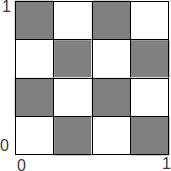
\includegraphics[width=0.2\textwidth]{plots/1_1.png}
    \caption{Checkerboard colouring for $n$=16}
  \end{center}
\end{figure}


\begin{figure}[!ht]
  \begin{center}
    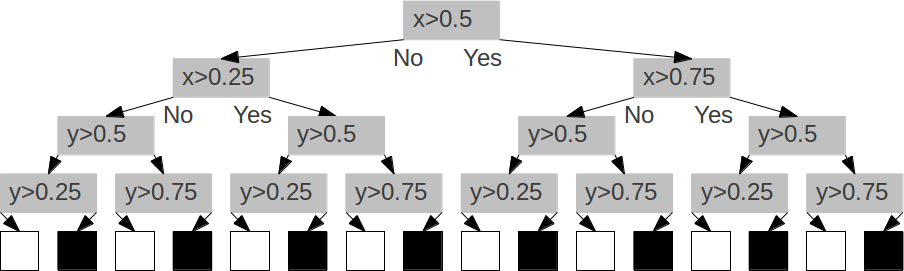
\includegraphics[width=0.60\textwidth]{plots/1_2.png}
    \caption{Decision tree for the scheme from Fig.1}
  \end{center}
\end{figure}


\textbf{Alternative argument} - ``quadtree''-like approach:\\
Suppose that the domain contains $n$ points. Then we can always split it in two s.t. each subdomain contains approximately the same number of points (to be precise, each subdomain contains at most $\frac{2^{\lceil\log_2n\rceil}}{2}$ points). Apply this recursively to each subdomain. We get a tree of depth at most $\lceil\log_2n\rceil$.

\section*{Problem 1.2}
Our worst case scenario in the solution of Problem 1.1 fulfills the requirements as the tree is of depth $n-1$.
